\documentclass[,a4paper,12pt,french]{article}

\usepackage[TD]{../../../StylePartage}

% Début du document
%%%%%%%%%%%%%%%%%%%
\begin{document}

\titre{Fonctions - Exercices}

\begin{exercice} \

On considère la fonction $\fonction f {[-5;5]} {\R} {x} {2x+4}$. Déterminer les images par $f$ de $-2$, $0$ et $3$.
\end{exercice}

\begin{exercice}
Pour chacune des fonctions ci-dessous, déterminer l'image de $2$:
\begin{enumerate}
\item $f:x \mapsto 4x^3-1$
\item $g:x \mapsto x^2-x-2$
\item $h:x \mapsto \frac{5x-2}{x+8}$
\item $i:x \mapsto x^4 - 2x(x+2)$
\end{enumerate}
\end{exercice}

\begin{exercice}
On considère trois fonctions $f$, $g$, $h$ définissant l'image du nombre $x$ de la manière suivante:

$ \hfill f(x)=6x+2 \hfill g(x)=x^2-x \hfill h(x)=\frac x {x+1} \hfill$

Compléter le tableau de valeurs suivant:

\begin{center}
\begin{tabularx}{0.8\linewidth}{|c|
	>{\Centering \arraybackslash}X|
	>{\Centering \arraybackslash}X|
	>{\Centering \arraybackslash}X|} \hline
$x$ & 0 & 1 & 2 \\ \hline
$f(x)$ & & & \rule{0pt}{8mm} \\ \hline
$g(x)$ & & & \rule{0pt}{8mm} \\ \hline
$h(x)$ & & & \rule{0pt}{8mm} \\ \hline
\end{tabularx}
\end{center}
\end{exercice}

\begin{exercice} \

\compo[0.4]
{
\begin{center}
Questions 2 à 4
\begin{tikzpicture}[scale=\echellepgf]
\begin{axis}[
styleglobal,
width=\echellepgfinv*\linewidth,
xmin=-3, xmax= 6,
ymin=-1.5, ymax=4.5,
xtick distance=1,
ytick distance=1,
]
\addplot[samples=101,smooth,line width=1.3pt,domain=(0:4),mark=none] plot coordinates {(-2,2) (-1,4) (1,0) (2,-1) (4,0) (5,2)};
\end{axis}
\end{tikzpicture}
\end{center}
}
{
On a représenté une fonction $f$ sur le repère ci-contre.
\begin{enumerate}
\item L'ensemble de définition de $f$ est $\dotfill$
\item L'image de 2 est \dotfill
\item L'image de -1 est \dotfill
\item L'image de 0 est \dotfill
\item 4 a pour antécédent(s) \dotfill
\item 1 a pour antécédent(s) \dotfill
\item -1 a pour antécédent(s) \dotfill
\item -2 a pour antécédent(s) \dotfill
\end{enumerate}
}

\vspace{5mm}

\compo[0.4]
{
\begin{center}
Questions 5 et 6
\begin{tikzpicture}[scale=4/5]
\begin{axis}[
styleglobal,
width=1.25*\linewidth,
xmin=-3, xmax= 6,
ymin=-1.5, ymax=4.5,
xtick distance=1,
ytick distance=1,
]
\addplot[samples=101,smooth,line width=1.3pt,domain=(0:4),mark=none] plot coordinates {(-2,2) (-1,4) (1,0) (2,-1) (4,0) (5,2)};
\end{axis}
\end{tikzpicture}
\end{center}
}
{
\begin{center}
\begin{minipage}[l]{0.66\linewidth} % Graphe à droite donc \linewidth correspond à 0.6 au lieu de 0.4 =>0.66
\Centering{Questions 7 et 8}
\begin{tikzpicture}[scale=4/5]
\begin{axis}[
styleglobal,
width=1.25*\linewidth,
xmin=-3, xmax= 6,
ymin=-1.5, ymax=4.5,
xtick distance=1,
ytick distance=1,
]
\addplot[styleplot,domain=(0:4)] plot coordinates {(-2,2) (-1,4) (1,0) (2,-1) (4,0) (5,2)};
\end{axis}
\end{tikzpicture}
\end{minipage}
\end{center}
}
\end{exercice}

\newpage

\begin{multicols*}{2}

\begin{exercice}
Soit $f$ la fonction définie par la courbe ci-dessous:

\Centering{
\begin{tikzpicture}[scale=\echellepgf]
\begin{axis}[
styleglobal,
width=0.9*\echellepgfinv*\linewidth,
xmin=-7, xmax= 7,
ymin=-3, ymax=5,
xtick distance=1,
ytick distance=1,
minor x tick num=0,
minor y tick num=0,
tick label style = {font=\scriptsize},
]
\addplot[styleplot] plot coordinates {(-6,3) (-5,1) (-3,-1) (-1,4) (1,3) (3,4) (4,2) (5,-1) (6,-2)};
\end{axis}
\end{tikzpicture}}
\begin{enumerate}
\item Déterminer les images par $f$ de $-5 \ , \ 3 \ , \ -1 \ , \ 1 \ , \ 4$.
\item Quel est le nombre d'antécédents par $f$ de $4 \ , \ 2 \ , \ 0 \ , \ -1 \ , \ -2 \ , \ 3$?
\item Parmi les points suivants, lesquels sont sur la courbe de $f$?
\compo[0.5]{\fakeitem $A(-2;1)$\\ \fakeitem $C(4;3)$}{\fakeitem $B(3;4)$\\ \fakeitem $D(-2;2)$}
\end{enumerate}
\end{exercice}

\begin{exercice} Soit $f:x \mapsto {2x-3}$.
\begin{enumerate}
\item On considère trois points $A,B,C$ sur la courbe de $f$, d'abscisses respectives $x_A=10 \ , \ x_B=1.2 \ , \ x_C=-\frac 1 4$. Calculer l'ordonnée de chacun de ces points.
\item Parmi les points suivants, lesquels sont sur la courbe de $f$?

$\hfill D(-3;0) \hfill E(7;11) \hfill F \left( \frac 3 2;0 \right) \hfill$
\item On considère trois points $A,B,C$ sur la courbe de $f$, d'ordonnées respectives $y_G=7 \ , \ y_H=-4,6 \ , \ h_I=\frac 1 2$. Calculer l'abscisse de chacun de ces points.
\end{enumerate}
\end{exercice}

\begin{exercice} \label{a corriger} \
On se donne la fonction $f$ définie sur $[-2;7]$ qui à $x$ associe $\frac {2x^3} {x^2+5x+15}$.
\begin{enumerate}
\item Réaliser le tableau de valeurs de $f$ entre $-2$ et $7$ par pas de $1$ à l'aide de la calculatrice. On arrondira au dixième près.
\item A l'aide de ce tableau de valeurs, tracer dans un repère la courbe représentative de $f$ sur $[-2;7]$.
\end{enumerate}
\end{exercice}

\columnbreak
\begin{exercice} \ %Pas fou, voir pour environnement itemize sur colonnes
\vspace{2mm}
\compobase{5pt}{c}{0.6}
{
$f$ est la fonction définie sur $\R^*=\R \setminus \{0 \}$ par: \vspace{-3mm}

$$f(x)=x-\frac 1 x \vspace{-1mm}$$

On a représenté $f$ dans le repère ci-contre. Parmi les points suivants, lesquels sont sur la courbe de $f$?
\compo[0.4]{\fakeitem $A(0;5)$}{\fakeitem $B(-2;-1.5)$}
\compo[0.4]{\fakeitem $C(1;0)$}{\fakeitem $D\left(4;\frac {15} 4 \right)$}
\compo[0.4]{\fakeitem $E(9;9)$}{\fakeitem $F(-5;4.8)$}
}
{
\begin{center}
\begin{tikzpicture}[scale=\echellepgf]
\begin{axis}[
styleglobal,
width=0.9*\echellepgfinv*\linewidth,
xmin=-3, xmax=3,
ymin=-4, ymax=4,
xtick distance=1,
ytick distance=1,
minor x tick num=0,
minor y tick num=0,
]
\addplot[styleplot,domain=(-4:4)] plot {x-1/x};
\end{axis}
\end{tikzpicture}
\end{center}
}
\end{exercice}

\begin{exercice}
Un coureur du tour de France a reporté sur le repère suivant sa distance parcourue en fonction du temps.

\Centering{
\begin{tikzpicture}[scale=\echellepgf]
\begin{axis}[
styleglobal,
hauteurproptick,
width=0.8*\echellepgfinv*\linewidth,
xmin=0, xmax= 4,
ymin=0, ymax=150,
xtick distance=1,
ytick distance=50,
minor x tick num=2,
minor y tick num=4,
ylabel={Distance parcourue (km)},
xlabel={Temps de course (h)},
label style={font=\normalsize},
]
\addplot[styleplot] plot coordinates {(0,0) (2/3,30) (1,50) (7/3,80) (8/3,90) (11/3,140)};
\end{axis}
\end{tikzpicture}}
\begin{enumerate}
\item Lire graphiquement la distance totale parcourue et la durée de la course.
\item Après combien d'heures de course le coureur a-t-il dépassé les 80km parcourus?
\end{enumerate}
\end{exercice}

\begin{exercice}
La courbe dans le repère ci-dessous représente la fonction $f$ qui à un instant $t$ exprimé en heures de l'intervalle $[0;24]$ associe la température $T$ en degrés Celsius, en un lieu.

\Centering{
\begin{tikzpicture}[scale=\echellepgf]
\begin{axis}[
styleglobal,
hauteurproptick,
width=0.8*\echellepgfinv*\linewidth,
xmin=0, xmax= 25,
ymin=-12, ymax=16,
xtick distance=2,
ytick distance=2,
minor x tick num=1,
minor y tick num=0,
ylabel={Température ($^{\circ}$C)},
xlabel={Temps (h)},
label style={font=\normalsize},
yscale=0.5,
]
\addplot[styleplot] plot coordinates {(0,10) (1,6) (2,2) (5,-4) (6,-8) (8,-10) (10,-8) (13,2) (15,8) (16,12) (18,14) (20,2) (24,-4)};
\end{axis}
\end{tikzpicture}}
\begin{enumerate}
\item Résoudre graphiquement l'équation $f(t)=2$. Interpréter le résultat.
\item Résoudre graphiquement l'inéquation $f(t) \geq -8$. Interpréter le résultat.
\end{enumerate}
\end{exercice}

\begin{exercice} \label{schemafonctions}
Dresser le tableau de variation et le tableau de signes des fonctions $f$, $g$ et $h$ définies sur le repère suivant:
\begin{centrer}
\begin{tikzpicture}[scale=\echellepgf]
\begin{axis}[
styleglobal,
width=0.8*\echellepgfinv*\linewidth,
xmin=-0.5, xmax= 8.5,
ymin=-2.5, ymax=3.5,
xtick distance=1,
ytick distance=1,
minor x tick num=1,
minor y tick num=1,
]
\addplot[styleplot,domain=(0:8)] plot {0.5*x-1.5)} node[pos=0.75,above] {$\mathscr C_f$};
\addplot[styleplot,color=DarkRed,densely dashed,domain=(0:8)] plot coordinates{(0,-2) (1,-1) (2,2) (3,3) (5,1) (6,0) (8,-2)} node[pos=0.6,above right] {$\mathscr C_g$};
\addplot[styleplot,densely dotted,color=DarkGreen,domain=(0:8)] plot coordinates{(0,3) (2,2) (3,0) (4,-2) (6,0) (7,2) (8,3)} node[pos=0.1,above right] {$\mathscr C_h$};
\end{axis}
\end{tikzpicture}
\end{centrer}
\end{exercice}

\begin{exercice}
Dresser le tableau de variation et le tableau de signes des fonctions de l'exercice 38.
\end{exercice}

\begin{exercice}
On se donne une fonction $f$ et son tableau de signes:
\begin{centrer}
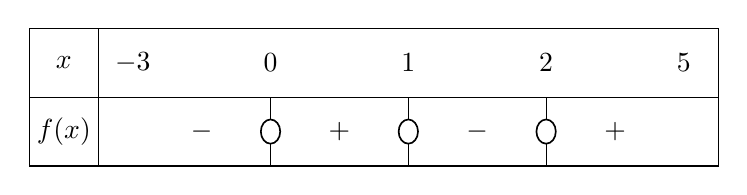
\begin{tikzpicture}[scale=0.875]
% Styles 
\tikzstyle{cadre}=[thin]
\tikzstyle{fleche}=[->,>=latex,thin]
\tikzstyle{nondefini}=[lightgray]
% Dimensions Modifiables
\def\Lrg{1}
\def\HtX{1}
\def\HtY{0.5}
% Dimensions Calculées
\def\lignex{-0.5*\HtX}
\def\lignef{-1.5*\HtX}
\def\separateur{-0.5*\Lrg}
% Largeur du tableau
\def\gauche{-1.5*\Lrg}
\def\droite{8.5*\Lrg}
% Hauteur du tableau
\def\haut{0.5*\HtX}
\def\bas{-2.5*\HtX-2*\HtY}
% Ligne de l'abscisse : x
\node at (-1*\Lrg,0) {$x$};
\node at (0*\Lrg,0) {$-3$};
\node at (2*\Lrg,0) {$0$};
\node at (4*\Lrg,0) {$1$};
\node at (6*\Lrg,0) {$2$};
\node at (8*\Lrg,0) {$5$};
% Ligne de la dérivée : f'(x)
\node at (-1*\Lrg,-1*\HtX) {$f(x)$};
\node at (0*\Lrg,-1*\HtX) {$ $};
\node at (1*\Lrg,-1*\HtX) {$-$};
\draw[cadre] (2*\Lrg,-0.5*\HtX) -- (2*\Lrg,-1.5*\HtX) node[pos=0.5,line width=0.6pt,draw=black,circle,minimum size=7pt,fill=white,inner sep=2pt,yscale=1.25] {};
\node at (3*\Lrg,-1*\HtX) {$+$};
\draw[cadre] (4*\Lrg,-0.5*\HtX) -- (4*\Lrg,-1.5*\HtX) node[pos=0.5,line width=0.6pt,draw=black,circle,minimum size=7pt,fill=white,inner sep=2pt,yscale=1.25] {};
\node at (5*\Lrg,-1*\HtX) {$-$};
\draw[cadre] (6*\Lrg,-0.5*\HtX) -- (6*\Lrg,-1.5*\HtX) node[pos=0.5,line width=0.6pt,draw=black,circle,minimum size=7pt,fill=white,inner sep=2pt,yscale=1.25] {};
\node at (7*\Lrg,-1*\HtX) {$+$};
\node at (8*\Lrg,-1*\HtX) {$ $};
% Ligne de la fonction : f(x)
% Encadrement
\draw[cadre] (\separateur,\haut) -- (\separateur, \lignef);
\draw[cadre] (\gauche,\haut) rectangle  (\droite, \lignef);
\draw[cadre] (\gauche,\lignex) -- (\droite,\lignex);
\end{tikzpicture}
\end{centrer}
\noindent Résoudre l'inéquation $f(x) \leq 0$.
\end{exercice}

\begin{exercice}
Parmi les fonctions représentées ci-dessous, lesquelles paraissent paires? Impaires? Ni l'un ni l'autre?

\noindent \begin{tabularx}{\linewidth}{
	>{\centering \arraybackslash}X
	>{\centering \arraybackslash}X}

\begin{tikzpicture}[scale=\echellepgf]
\begin{axis}[
styleglobal,
width=0.9*\echellepgfinv*\linewidth,
xmin=-3, xmax= 3,
ymin=-2.5, ymax=2.5,
xtick distance=1,
ytick distance=1,
minor x tick num=0,
minor y tick num=0,
]
\addplot[styleplot,domain=(-2.5:2.5)] plot {2*sin(deg(2*x))} node[pos=0.7,right] {$\mathscr C_f$} \pointsextremites;
\end{axis}
\end{tikzpicture}
&
\begin{tikzpicture}[scale=\echellepgf]
\begin{axis}[
styleglobal,
width=0.9*\echellepgfinv*\linewidth,
xmin=-3, xmax= 3,
ymin=-1, ymax=4,
xtick distance=1,
ytick distance=1,
minor x tick num=0,
minor y tick num=0,
]
\addplot[styleplot,domain=(-4:4)] plot {0.5*x^2-0.5} node[pos=0.65,right] {$\mathscr C_g$};
\end{axis}
\end{tikzpicture}
\\
\begin{tikzpicture}[scale=\echellepgf]
\begin{axis}[
styleglobal,
width=0.9*\echellepgfinv*\linewidth,
xmin=-3, xmax= 3,
ymin=-2, ymax=3,
xtick distance=1,
ytick distance=1,
minor x tick num=0,
minor y tick num=0,
]
\addplot[styleplot,domain=(-4:2)] plot {e^x-1.5} node[pos=0.6,right] {$\mathscr C_h$};
\end{axis}
\end{tikzpicture}
&
\begin{tikzpicture}[scale=\echellepgf]
\begin{axis}[
styleglobal,
width=0.9*\echellepgfinv*\linewidth,
xmin=-15, xmax= 15,
ymin=-12.5, ymax=12.5,
xtick distance=5,
ytick distance=5,
minor x tick num=0,
minor y tick num=0,
]
\addplot[styleplot,domain=(-12:12)] plot {0.01*x^3} node[pos=0.75,right] {$\mathscr C_i$};
\end{axis}
\end{tikzpicture}
\\
\begin{tikzpicture}[scale=\echellepgf]
\begin{axis}[
styleglobal,
width=0.9*\echellepgfinv*\linewidth,
xmin=-6, xmax= 6,
ymin=-2, ymax=8,
xtick distance=2,
ytick distance=2,
minor x tick num=0,
minor y tick num=0,
]
\addplot[styleplot,domain=(-10:10)] plot {5.5*e^(-(0.4*x)^2)} node[pos=0.7,above right] {$\mathscr C_j$};
\end{axis}
\end{tikzpicture}
&
\begin{tikzpicture}[scale=\echellepgf]
\begin{axis}[
styleglobal,
width=0.9*\echellepgfinv*\linewidth,
xmin=-3, xmax= 3,
ymin=-1, ymax=4,
xtick distance=1,
ytick distance=1,
minor x tick num=0,
minor y tick num=0,
]
\addplot[styleplot,domain=(-4:4)] plot {abs(x)} node[pos=0.75,below right] {$\mathscr C_k$};
\end{axis}
\end{tikzpicture}
\\
\end{tabularx}
\end{exercice}

\begin{exercice} \vspace{-2mm}
On se donne les fonctions $f,g,h,i$ suivantes:

\begin{itemize}
\item $\ f(x)-3x^2-10$ sur $\R$
\item $\ g(x)=x^3-2x+7$ sur $\R$
\item $\ h(x)=\frac 4 {x^3}$ sur $\R^*=\R \setminus \{0 \}$
\item $\ i(x)=\frac 3 {x^2-4}$ sur $[-1;1]$
\end{itemize}

\begin{enumerate}
\item Afficher leur courbe représentative à l'aide de la calculatrice, et conjecturer leur parité.
\item Démontrer la conjecture en calculant $f(-x)$.
\end{enumerate}
\end{exercice}

\begin{exercice}
Soit $f$ une fonction définie sur $[-4;4]$, telle que $f(-2)=3$ et $f(2)=4$. Que dire de la parité de cette fonction?
\end{exercice}

\begin{exercice}
Compléter la représentation graphique des fonctions suivantes afin d'obtenir une fonction paire en rouge, et une fonction impaire en bleu:

\compo[0.5]
{
\begin{tikzpicture}[scale=\echellepgf]
\begin{axis}[
styleglobal,
width=0.9*\echellepgfinv*\linewidth,
xmin=-3, xmax= 3,
ymin=-3, ymax=3,
xtick distance=1,
ytick distance=1,
minor x tick num=0,
minor y tick num=0,
]
\addplot[styleplot,domain=(0:3)] plot {2-2*e^(-(0.8*x)^2)};
\end{axis}
\end{tikzpicture}
}
{
\begin{tikzpicture}[scale=\echellepgf]
\begin{axis}[
styleglobal,
width=0.9*\echellepgfinv*\linewidth,
xmin=-3, xmax= 3,
ymin=-3, ymax=3,
xtick distance=1,
ytick distance=1,
minor x tick num=0,
minor y tick num=0,
]
\addplot[styleplot,domain=(-4:0)] plot coordinates {(-3,3) (-1,-1) (0,0)};
\end{axis}
\end{tikzpicture}
}
\end{exercice}

\begin{exercice}[*]
On a représenté deux fonctions $f$ et $g$ sur le repère ci-dessous:
\begin{centrer}
\begin{tikzpicture}[scale=\echellepgf]
\begin{axis}[
styleglobal,
width=0.8*\echellepgfinv*\linewidth,
xmin=-3.5, xmax= 3.5,
ymin=-2, ymax=2,
xtick distance=1,
ytick distance=1,
minor x tick num=1,
minor y tick num=1,
]
\addplot[styleplot,domain=(-3:3)] plot {0.8*sin(4*deg(x))*(e^(-0.5*x^2)+1)} node[pos=0.6,above right] {$\mathscr C_f$} \pointsextremites;
\addplot[styleplot,densely dashed,domain=(-3:3),color=DarkBlue] plot {0.3*x} node[pos=0.95,above] {$\mathscr C_g$} \pointsextremites;
\end{axis}
\end{tikzpicture}
\end{centrer}
\noindent Résoudre les (in)équations suivantes:
\begin{enumerate}
\item $f(x) = 1 $
\item $f(x) < g(x)$
\item $f(x) \leq h(x) \leq g(x)$
\end{enumerate}
\end{exercice}

\begin{exercice}[*]
Soit $f$ une fonction définie sur $[0;8]$. Voici l'ensemble des solutions de certaines inéquations:
\vspace{2mm}
\begin{centrer}
\begin{minipage}{0.7\linewidth}
\compo[0.5]{\fakeitem $f(x) \geq 1$} {$\mathscr S=[0;8]$}
\compo[0.5]{\fakeitem $f(x)>1$} {$\mathscr S=]0;8[$}
\compo[0.5]{\fakeitem $f(x)\geq 2$} {$\mathscr S=[3;6]$}
\compo[0.5]{\fakeitem $f(x) \geq 3$} {$\mathscr S=[3,5;5]$}
\compo[0.5]{\fakeitem $f(x) \geq 4$} {$\mathscr S=\{4 \}$}
\end{minipage}
\end{centrer}
\vspace{2mm}
Dans un repère, tracer une courbe susceptible de représenter la fonction $f$.
\end{exercice}

\begin{exercice}[*]
On reprend les trois fonctions de l'exercice \ref{schemafonctions}. Dans chaque cas, résoudre:
\begin{enumerate}
\item $f(x) \leq g(x) \leq h(x)$
\item $h(x) \leq g(x) \leq f(x)$
\item $f(x) \leq h(x) \leq g(x)$
\end{enumerate}
\end{exercice}

\begin{exercice}[*]
On se donne une fonction $f$ définie sur $[-5;4]$. On a dressé son tableau de variations et son tableau de signes ci-dessous:
\begin{centrer}
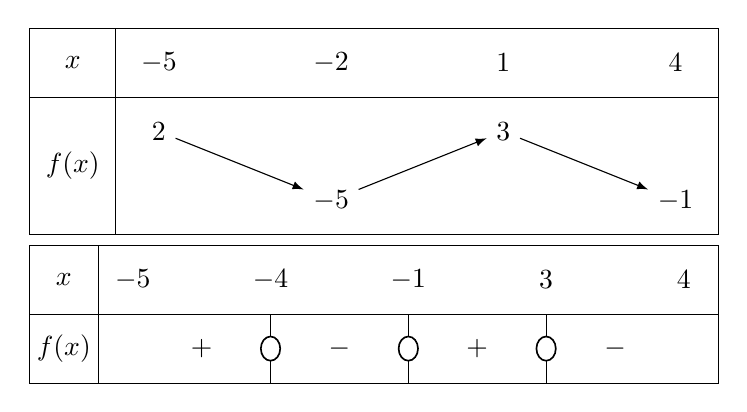
\begin{tikzpicture}[scale=0.875]
% Styles 
\tikzstyle{cadre}=[thin]
\tikzstyle{fleche}=[->,>=latex,thin]
\tikzstyle{nondefini}=[lightgray]
% Dimensions Modifiables
\def\Lrg{5/4}
\def\HtX{1}
\def\HtY{0.5}
% Dimensions Calculées
\def\lignex{-0.5*\HtX}
\def\lignef{-1.5*\HtX}
\def\separateur{-0.5*\Lrg}
% Largeur du tableau
\def\gauche{-1.5*\Lrg}
\def\droite{6.5*\Lrg}
% Hauteur du tableau
\def\haut{0.5*\HtX}
\def\bas{-1.5*\HtX-2*\HtY}
% Ligne de l'abscisse : x
\node at (-1*\Lrg,0) {$x$};
\node at (0*\Lrg,0) {$-5$};
\node at (2*\Lrg,0) {$-2$};
\node at (4*\Lrg,0) {$1$};
\node at (6*\Lrg,0) {$4$};
% Ligne de la fonction : f(x)
\node  at (-1*\Lrg,{-1*\HtX+(-1)*\HtY}) {$f(x)$};
\node (f1) at (0*\Lrg,{-1*\HtX+(0)*\HtY}) {$2$};
\node (f2) at (2*\Lrg,{-1*\HtX+(-2)*\HtY}) {$-5$};
\node (f3) at (4*\Lrg,{-1*\HtX+(0)*\HtY}) {$3$};
\node (f4) at (6*\Lrg,{-1*\HtX+(-2)*\HtY}) {$-1$};
% Flèches
\draw[fleche] (f1) -- (f2);
\draw[fleche] (f2) -- (f3);
\draw[fleche] (f3) -- (f4);
% Encadrement
\draw[cadre] (\separateur,\haut) -- (\separateur,\bas);
\draw[cadre] (\gauche,\haut) rectangle  (\droite,\bas);
\draw[cadre] (\gauche,\lignex) -- (\droite,\lignex);

\begin{scope}[shift= {(-0.38,-3.15)}]
% Styles 
\tikzstyle{cadre}=[thin]
\tikzstyle{fleche}=[->,>=latex,thin]
\tikzstyle{nondefini}=[lightgray]
% Dimensions Modifiables
\def\Lrg{1}
\def\HtX{1}
\def\HtY{0.5}
% Dimensions Calculées
\def\lignex{-0.5*\HtX}
\def\lignef{-1.5*\HtX}
\def\separateur{-0.5*\Lrg}
% Largeur du tableau
\def\gauche{-1.5*\Lrg}
\def\droite{8.5*\Lrg}
% Hauteur du tableau
\def\haut{0.5*\HtX}
\def\bas{-2.5*\HtX-2*\HtY}
% Ligne de l'abscisse : x
\node at (-1*\Lrg,0) {$x$};
\node at (0*\Lrg,0) {$-5$};
\node at (2*\Lrg,0) {$-4$};
\node at (4*\Lrg,0) {$-1$};
\node at (6*\Lrg,0) {$3$};
\node at (8*\Lrg,0) {$4$};
% Ligne de la dérivée : f'(x)
\node at (-1*\Lrg,-1*\HtX) {$f(x)$};
\node at (0*\Lrg,-1*\HtX) {$ $};
\node at (1*\Lrg,-1*\HtX) {$+$};
\draw[cadre] (2*\Lrg,-0.5*\HtX) -- (2*\Lrg,-1.5*\HtX) node[pos=0.5,line width=0.6pt,draw=black,circle,minimum size=7pt,fill=white,inner sep=2pt,yscale=1.25] {};
\node at (3*\Lrg,-1*\HtX) {$-$};
\draw[cadre] (4*\Lrg,-0.5*\HtX) -- (4*\Lrg,-1.5*\HtX) node[pos=0.5,line width=0.6pt,draw=black,circle,minimum size=7pt,fill=white,inner sep=2pt,yscale=1.25] {};
\node at (5*\Lrg,-1*\HtX) {$+$};
\draw[cadre] (6*\Lrg,-0.5*\HtX) -- (6*\Lrg,-1.5*\HtX) node[pos=0.5,line width=0.6pt,draw=black,circle,minimum size=7pt,fill=white,inner sep=2pt,yscale=1.25] {};
\node at (7*\Lrg,-1*\HtX) {$-$};
\node at (8*\Lrg,-1*\HtX) {$ $};
% Ligne de la fonction : f(x)
% Encadrement
\draw[cadre] (\separateur,\haut) -- (\separateur, \lignef);
\draw[cadre] (\gauche,\haut) rectangle  (\droite, \lignef);
\draw[cadre] (\gauche,\lignex) -- (\droite,\lignex);
\end{scope}
\end{tikzpicture}
\end{centrer}
\noindent Tracer dans un repère une courbe représentative potentielle de $f$.
\end{exercice}

\begin{exercice}[*]
Soit $f$ une fonction impaire. Que dire de $f(0)$?
\end{exercice}

\begin{exercice}[*]
Soit $f$ une fonction paire telle que $f(3)=1$ et telle que l'équation $f(x)=4$ admet $1$ et $4$ pour solutions dans $[ 0 ; + \infty ]$. Donner:
\begin{enumerate}
\item L'image de $-3$ par $f$.
\item Les solutions de l'équation $f(x)=4$ dans $\R$.
\end{enumerate}
\end{exercice}

\newpage

\end{multicols*}

\newpage

\titre{Corrections}

\begin{Large}
\textbf{Exercice \ref{a corriger}.}

\begin{center}
\begin{tabularx}{0.9\linewidth}{|c|
	>{\Centering \arraybackslash}X|
	>{\Centering \arraybackslash}X|
	>{\Centering \arraybackslash}X|
	>{\Centering \arraybackslash}X|
	>{\Centering \arraybackslash}X|
	>{\Centering \arraybackslash}X|
	>{\Centering \arraybackslash}X|
	>{\Centering \arraybackslash}X|
	>{\Centering \arraybackslash}X|
	>{\Centering \arraybackslash}X|} \hline
$x$ & $-2$ & $-1$ & $0$ & $1$ & $2$ & $3$ & $4$ & $5$ & $6$ & $7$ \\ \hline
$f(x)$ & & & & & & & & & & \rule{0pt}{8mm} \\ \hline
\end{tabularx}

\begin{tikzpicture}[scale=\echellepgf]
\begin{axis}[
styleglobal,
labelgros,
width=0.9*\echellepgfinv*\linewidth,
xmin=-3, xmax= 8,
ymin=-3, ymax=8,
xtick distance=1,
ytick distance=1,
]

\end{axis}
\end{tikzpicture}
\end{center}

\end{Large}
\end{document}
